\section{Sistemas de Radiocomunicación por Satélite}
\label{sec:satelite}
	\subsection{Introducción e historia}
	\label{sub:introSat}
		El objetivo delos sistemas de radiocomunicación por satelite es el establecimiento de enlaces entre estaciones, tanto fijas como móviles, mediante repetidores en la órbita terrestre. Este concepto se refleja ya en artículos desde 1929. Los repetidores pueden ser tanto activos como pasivos, es decir, pueden amplificar la señal o no.\\
		La carrera espacial empieza con la idea de utilizar el espacio para lo militar. En 1957 se lanzan los primeros Sputnik y a Laika. Mientras tanto en estados unidos crean la NASA, sin lanzar nada al espacio. A partir de 1958 se empiezan a lanzar satelites de comunicación de la NASA con el departamento de defensa yanki. El primero fue un repetidor pasivo. En 1963 se pone en orbita el primer satélite geoestacionario, el Syncom 2.\\
		En 1964 se crea INTELSAT, una organización de 11 paises para la creación de un sistema comercial mundial de telecomunicaciones vía satélite. En la actualidad es privado y lo componen 109 paises. El primer satélite fue el early bird (INTELSAT I).\\
		Los sistemas satélite son una alternativa a otros sistemas. Con 3 satélites geoestacionarios se puede cubrir toda la superficie terrestre. Los equipos de comunicación y control deben ser muy fiables, ya que, la reparación puede ser imposible, además de estar expuestos a gran cantidad de radiaciones. Tienen una vida util limitada por el fin del combustible usado para los motores, una vez sin combustible no se pueden reorientar y se envian a una órbita basura. Los sistemas satélite se suelen usar como complemento, por ejemplo, un cable submarino puede tener un sistema satélite de soporte.
	% subsection introSat (end)
	\subsection{Servicios de satélites}
	\label{sub:serviciosSat}
		\begin{itemize}
			\item Servicio fijo: Enlaces entre dos puntos terrestres usando el satélite como repetidor.
			\item Servicio Móvil: Uno o más puntos fijos y móviles, como barcos, aviones y torres de control.
			\item Servicio de radiodifusión: Uno o más puntos fijos y terminales dispersos, como la televisión o la radio satélite.
			\item Servicio de radiodeterminación: Localización determinada por satélites, como los sistemas \acrshort{GPS} o Galileo.
			\item Servicio de exploración de la tierra: desde mapas del tiempo (meteosat), creación de mapas hasta la exploración de recursos.
			\item Servicio de exploración del espacio: mediante el uso de telescopios o radiotelescopios como el Hubble.
			\item Servicio entre satélites: La comunicación entre satélites no tiene limitaciones físicas para el uso de ancho de banda, por ejemplo, a 60GHz el oxígeno absorbe la señal, en el espacio no.
		\end{itemize}
	% subsection serviciosSat (end)
	\subsection{Estructura del sistema de comunicación satélite}
	\label{sub:estructSat}
		\begin{figure}[H]
			\centering
			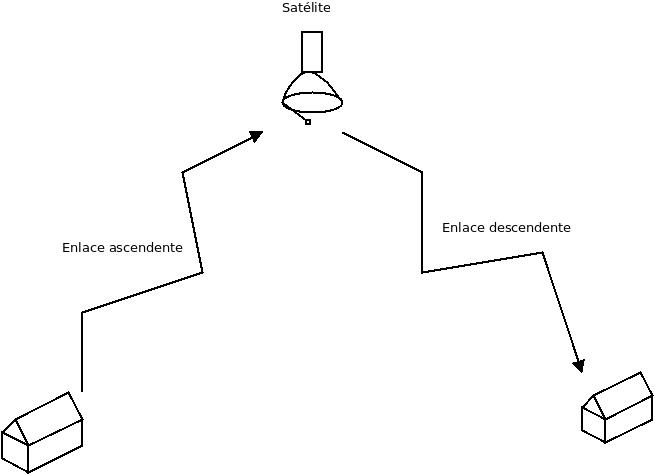
\includegraphics[width=0.7\textwidth]{Imagen/arquisatelite.jpg}
			\caption{Estructura de un sistema de comunicación satélite}
		\end{figure}
		\begin{itemize}
			\item Estación terrena de transmisión: Recibe la señal para posteriormente modularla a una radiofrecuencia (\acrshort{RF}), amplificarla y después transmitirla. En transmisión se necesita mucha potencia y una gran directividad.
			\item Enlaces: tanto el enlace ascendente como el descendente se modelan como sistemas de transmisión en espacio libre con pérdidas ocasionadas por la frecuencia, distancia, atmosfera e incluso la lluvia.
			\item Satélite: Se trata de una estación repetidora, que amplifica, cambia de banda y retransmite las señales. Las partes involucradas en cada acción vienen descritas a continuación:
			\begin{itemize}
				\item Recepción: La antena, un filtro y un amplificador de bajo ruido.
				\item Transpondedor: Se trata de un conversor de frecuencia y amplificador encargado de llevar a cabo la retransmisión.
				\item Conmutación: piezas encargadas del encaminamiento y por tanto de la asignación de transpondedores.
				\item Transmisión: Amplificación, filtrado y antena de transmisión.
			\end{itemize}
			\item Estación terrena de recepción: Hace uso de un recptor superheterodino, receptor de ondas de radio que utiliza un proceso de mezcla de frecuencias o heterodinación para convertir la señal recibida en una a frecuencia intermedia. Esta señal sin la radioportadora de alta frecuencia es mucho más facil de manejar que la original.
			\item Segmento espacial: La suma de los retardos en los enlaces, en transmisión, en recepción y en el satélites terminan produciendo grandes retardos, 250ms en geoestacionarios. Este hecho hace necesario el uso de técnicas de cancelación de ecos.
		\end{itemize}
		El diseño de estos sistemas de comunicación satélite tiene que tener en cuenta los siguientes aspectos:
		\begin{itemize}
			\item Órbita: En la mayoría de las ocasiones se utiliza una órbita geoestacionaria. Para comunicaciones móviles se empiezan a utilizar órbitas meo y leo para reducir el retardo y la potencia transmitida.
			\item Cobertura: Se pueden usar varios transpondedores para poder conformar un haz de diferente tipo y anchura.
			\item Conectividad: Capacidad de establecer enlaces entre estaciones terrenas. 
			\item Técnicas de acceso múltiple para la compartición del satélite. Se suelen utilizar \acrshort{FDMA} y \acrshort{TDMA}, en algunas ocasiones se puede utilizar CDMA pero supone un gran problema.
			\item Banda de frecuencia y ancho de banda: Se utilizan diferentes bandas según el servicio y la disponibilidad necesitada. Las bandas a mayor frecuencia han de transmitir más potencia para superar la peor propagación. Para aumentar la reutilización se separan haces de la misma frecuencia polarizandolos opuestos. Para aumentar aún más la eficiencia se mejoran el tratamiento de la señal y las modulaciones.
			\item Potencia: Se busca un compromiso entre la distancia a recorrer y la limitación a bordo del satélite. Una nueva limitación es la interferencia con otros satélites y estaciones terrenas.
		\end{itemize}
	% subsection estructSat (end)
	\subsection{Órbitas}
	\label{sub:orbitas}
		Las óbitas se basan en las leyes de Kepler, consecuencia de la ley de gravitación universal. La elección de la órbita depende del tipo de cobertura, aplicación o recursos económicos. Las órbitas disponibles son escasas. Existen dos tipos de órbitas, las geoestacionarias y las oblícuas. Las órbitras geoestacionarias (\acrshort{GEO}) son órbitas circulares, en una latitud baja, inclinación nula y un periodo de revolución igual al ciclo terrestre. Estos satélites siempre son visibles y no requieren, teoricamente, de un seguimiento. En las órbitas oblicuas, en cambio, el seguimiento ha de ser continuo, ya que el satélite sale y se pone. Dependiendo de la altura de la órbita puede ser: baja (\acrshort{LEO}), media (\acrshort{MEO}) o alta (\acrshort{HEO}). Tanto los \acrshort{LEO} como los \acrshort{MEO} son más baratos de lanzar que los \acrshort{GEO}.\\
		Las ventajas de las órbitas de tipo geoestacionaria son, la gran superficie de cobertura y permiten la existencia de estaciones terrenas fijas. Las mayores desventajas son la potencia necesaria para la transmisión, las antenas necesarias, los retardos, los lanzamientos de alto coste y la imposibilidad que presentan de cubrir latitudes altas.
		La órbita geoestacionaria viene definida por la siguiente formula, tomando los siguientes valores. $\omega=\frac{2\pi}{T}$ para un periodo de rotación T=23h 56min.
		\[G\frac{Mm}{d^2}=md\omega^2\]
		De esta formula y teniendo en cuenta un radio de la tierra de 6366km, se obtiene una distancia a la superficie de la tierra de 35806km.\\
		La cobertura del satélite tiene dos formas, la cobertura geométrica es la cobertura real que ofrece el satélite, esta es diferente de la cobertura radioeléctrica. La cobertura radioélectrica es igual a la geométrica pero tiene en cuenta el ruido terrestre y los obstáculos físicos, es decir es una cobertura real.
	% subsection orbitas (end)
	\subsection{Distancias satelitales}
	\label{sub:distSatelite}
		Las coordenadas cartesianas del satélite son las siguientes: 
		\begin{gather*}
			x_s=R+h\\
			y_s=0\\
			z_s=0
		\end{gather*}
		Las coordenadas de la estación terrena, en cambio:
		\begin{gather*}
			x_e=Rcos\phi cos\lambda\\
			y_e=Rsin\phi cos\lambda\\
			z_e=Rsin\lambda
		\end{gather*}
		Los ángulos $\phi$ y $\lambda$ son longitud y latitud. $\phi$ se calcula como la diferencia entre la longitud del satélite y la longitud de la estación terrena. $\phi_l=\phi_s-\phi_e$. El ángulo $\lambda$ es la latitud de la estación terrena, ya que, la latitud del satélite, al estar sobre el ecuador es 0.\\
		La distancia entre el satélite y la estación terrena se puede calcular por medio de una simple regla de pitagoras:
		\begin{equation}
			\tag{Distancia al satélite}
			ES=d=\sqrt{(x_s-x_e)^2+y_e^2+z_e^2}=\sqrt{(R+h)^2+R^2-2R(R+h)cos\phi cos\lambda}
		\end{equation}
	% subsection distSatelite (end)
	\subsection{Carga util del satélite}
	\label{sub:satUtil}
		\subsubsection{Transpondedor}
		\label{ssub:transpondedor}
			El transpondedor es la parte del satélite que realiza la conversión de frecuencias y la amplificación de la señal. El ancho de banda es algo que depende de la función de las señales y técnicas de acceso múltiple utilizadas. Las características de un transpondedor general son las siguientes:
			\begin{itemize}
				\item La respuesta a una frecuencia plana conlleva una respuesta plana en amplitud, es decir, el tranpondedor siempre trabaja en su zona lineal.
				\item El retardo de grupo se mantiene constante.
				\item La linealidad de la respuesta en potencia se define como back-off. El back-off es el cociente entre la potencia de entrada y la potencia de salida.
			\end{itemize}
			Los transpondedores regenerativos son una mejora sobre los regeneradores pasivos. A diferencia de los pasivos, los transpondedores regenerativos evitan la degradación por falta de linealidad. La mayor diferencia es que los transpondedores regenerativos demoludan la señal y la remodulan con más potencia. De esta forma se puede independizar los enlaces ascendente y descendente.
		
		% subsubsection transpondedor (end)
		\subsubsection{Antenas}
		\label{ssub:antenas}
		A lo largo de la historia de los satélites se han utilizado diferentes tipos de antena. Antenas de hilo (monopolos, dipolos) se utilizan para TTC omnidireccionales. Lo siguiente fueron las bocinas, tienen un haz ancho con cobertura global. Las antenas reflectoras tienen un haz más estrecho y se suele utilizar en sistemas con arrays. Cada una de ellas produce esquemas de cobertura diferentes, ya sean de cobertura omnidireccional, global, hemisférica o de haz.
		% subsubsection antenas (end)
	% subsection satUtil (end)
	\subsection{Acceso múltiple}
	\label{sub:satAccesoMultiple}
		En el trayecto ascendente cada estación terrena accede individualmente al satélite. El trayecto descendente suele usarse la difusión y cada una de las estaciones terrenas extrae la señal destinada a ella. El satélite realiza la traslación de frecuencias, amplificación y filtrado de las señales para la retransmisión. En los sistemas satélite comercial se usan 2 tecnicas de acceso múltiple: \acrshort{FDMA} y \acrshort{TDMA}.\\
		En \acrshort{FDMA} se distribuye el ancho de banda entre las estaciones participantes. Esto produce un nivel de interferencia entre estaciones muy pequeña. El transpondedor hace la conversación de frecuencias y amplificación. Esto produce un problema de ruido de intermodulación en el amplificador. El enlace descendente difunde toda la banda y la estación terrena recibe toda para a continuación sintonizar las portadoras destinadas a ella.\\
		En \acrshort{TDMA} la información debe ser digital. Hay que mantener tiempos de guarda para compensar la diferencia en los tiempos de llegada al satélite. \acrshort{TDMA} solo se usa en el sentido ascendente, para el sentido descendente se transmiten las señales con multiplex por división en tiempo. El número de intervalos por trama varía entre 3 y 100, variando la duración de las tramas en consecuencia.
		El \acrshort{FDMA} es más facil de realizar y no requiere de temporización. El \acrshort{TDMA}, en cambio, utiliza toda la potencia disponible, es más flexible y además es digital controlando errores y con modulaciones digitales. Como contra, en \acrshort{TDMA} la temporización es muy estricta y mantiene un retardo añadido al ser una transmisión discontinua. El mayor contra del \acrshort{FDMA} es el ruido intermodulación que se produce entre las portadoras, esto reduce el tiempo de trabajo del amplificador.
	% subsection satAccesoMultiple (end)
	\subsection{Balance de Enlace}
	\label{sub:balance}
		Es el calculo de potencias que permite determinar la calidad de un enlace. El balance del enlace se puede generalizar con la siguiente formula.
		\begin{equation}
			\tag{Balance de enlace}
			\frac{c}{N_0}=P_{tx}+G_{tx}+\frac{G_{rx}}{T}-L-BO-10logKB
		\end{equation}
		De la fórmula sabemos que T es la temperatura del receptor, K es la constante de Boltzman, B el ancho de banda del canal, L son las pérdidas del enlace, BO es el Back-Off. El back-Off se diferencia en: Input Back-Off para el sentido ascendente y Output Back-Off para el descendente, \acrshort{IBO} y \acrshort{OBO}. El factor de calidad del enlace es el cociente entre la ganancia y temperatura del receptor.\\
		La calidad del enlace para enlaces digitales se calcula de la siguiente forma:
		\begin{equation}
			\tag{Balance de enlace digital}
			\frac{e_b}{n_0}=\frac{c}{n_0}\frac{1}{R_b}
		\end{equation}
	% subsection balance (end)
	\subsection{Redes Very Small Aperture Terminals (\acrshort{VSAT})}
	\label{sub:vsat}
		Redes de comunicaciones por satélite que proporcionan servicios FSS y que utilizan estaciones pequeñas en las instalaciones del usuario. Proporcionan conexiones entre terminales remotos y una estación terminal (HUB). Los sistemas \acrshort{VSAT} tienen como principales ventajas el acceso a puntos remotos, una gran calidad, facilidad de crecimiento de la red, adaptatividad y unos costes bajos de realización.
		\begin{figure}[H]
		\centering
		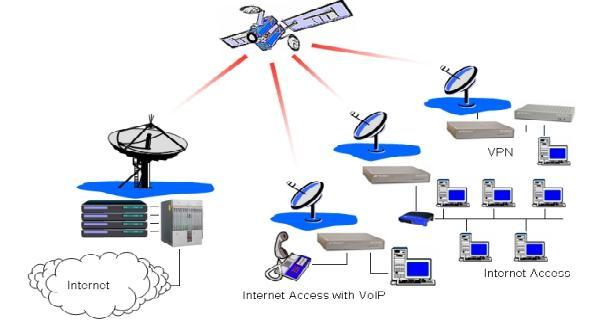
\includegraphics[width=\textwidth]{Imagen/diavsat.jpg}
		\caption{Diagrama de una red \acrshort{VSAT}}
		\end{figure}
		El enlace inbound se define como el enlace en sentido terminal remoto$\to$HUB pasando por el satélite. El sentido outbound al ser un sistema multicast desde un único punto se utiliza duplexación o en tiempo(TDM) o en frecuencia(FDM). El sentido inbound es el único que utiliza técnicas de multiplexación. Estas técnicas pueden permitir el acceso aleatorio con aloha, aloha ranurado, la asignación bajo demanda de los recursos, o incluso la asignación fija de recursos. La utilización de las diferentes formas de asignación variarán dependiendo de la conformación del tráfico utilizado, rafagas cortas, tráfico interno o tráfico continuo.
	% subsection vsat (end)
	\subsection{Comunicaciones móviles por satélite}
	\label{sub:satMovil}
		En comunicaciones móviles por satélite se utilizan dos tipos de órbita, de baja altura o geoestacionarios. Los costes son menores en órbita baja pero la cobertura en los polos se hace imposible.\\
		El campo de visión de la superficie terrestre es limitado en órbitas bajas, con lo cual hace falta gran cantidad de satélites organizados para dar una cobertura ancha. Las órbitas \acrshort{LEO} pueden ser circulares o elípticas, polares o inclinadas. Para el cálculo de las características de las órbitas \acrshort{LEO} supondremos órbitas circulares, el radio de la tierra lo supondremos 6377km, el radio de la órbita lo definiremos como a y la constante de keppler $k=Gm_E=3.98601352*10^5\sfrac{km^3}{seg^2}$.
		\begin{equation}
			\tag{Velocidad lineal}
			v_s=\sqrt{k(\frac{2}{r_E+h})}=\sqrt{\frac{k}{r_E+h}}
		\end{equation}
		\begin{equation}
			\tag{Velocidad angular}
			\omega_s=\frac{v_s}{r_E+h}=\sqrt{\frac{k}{(r_E+h)^3}}
		\end{equation}
		Esto nos da un periodo orbital de:
		\begin{equation}
			\tag{Periodo orbital}
			T_s=2\pi\sqrt{\frac{(r_E+h)^3}{k}}
		\end{equation}
		Para calcular el angulo central en el borde de cobertura, el ángulo que forma el satélite con la estación terrena visto desde el centro de la tierra, se puede hacer en función del ángulo de elevación mínima.
		\begin{equation}
			\tag{Ángulo central}
			\gamma=arccos(\frac{r_E}{r_E+h}cosEl)-El
		\end{equation}
		La distancia desde el borde de cobertura del satélite será la siguiente:
		\begin{equation}
			\tag{Distancia al satélite}
			d=\sqrt{r_E^2+(r_E+h)^2-2r_E(r_E+h)cos\gamma}
		\end{equation}
		El área del casquete de cobertura nos permitirá calcular el número mínimo de satelites necesarios.
		\begin{equation}
			\tag{Número de satélites}
			N=\frac{4\pi r_E^2}{S}=\frac{2}{1-cos\gamma}
		\end{equation}
	% subsection satMovil (end)
	\subsection{Sistemas de navegación por satélite \acrshort{GPS}}
\label{sub:gps}
	A partir de las distancias entre 3 satélites y el receptor, conocidas las posiciones de los satélites, se puede calcular la posición del receptor. La mayor parte del error se debe a la deriva existente entre el reloj del satélite y del receptor. Otras fuentes de error son los efectos de la propagación en las diferentes capas de la atmósfera.\\
	Existen dos códigos diferenciados para la localización según la precisión necesaria. El código P y los códigos C/A. Los primeros, mucho más precisos, se utilizan en aplicaciones militares y los segundos en aplicaciones comerciales.
% subsection gps (end)
% section satelite (end)